\chapter{Diskuse a výsledky}
\section{Průchod aplikacemi}
Tyto průchody aplikacemi demonstrují všechny funkce aplikací a ukazují celý cyklus od vytvoření projektu přes vizualizaci až po zpětnou vazbu, což naplňuje cíl práce.

\subsection{Webové rozhraní}
Celý proces začíná na webovém rozhraní. Hlavní stránka zobrazuje přehled projektů ve formě karet obsahujících náhledový obrázek, název, popis, souřadnice, průměrné hodnocení a tlačítka pro správu. viz. obrázek \ref{fig:web}

\begin{figure}[H]
    \centering
    \includegraphics[width=\textwidth]{images/web_overview.png}
    \caption{Webové administrátorské rozhraní s přehledem projektů}
    \label{fig:web}
\end{figure}

\pagebreak

Uživatel vytvoří nový projekt kliknutím na tlačítko pro přidání, čímž se otevře modální formulář. Vyplní název, popis a souřadnice, nahraje GLB soubor s 3D modelem a náhledový obrázek. Po uložení je projekt validován a okamžitě zpřístupněn v mobilní aplikaci. viz. obrázek \ref{fig:web_add}

\begin{figure}[H]
    \centering
    \includegraphics[width=0.86\textwidth]{images/web_add.png}
    \caption{Formulář pro přidání nového projektu}
    \label{fig:web_add}
\end{figure}

Uživatel může projekt průběžně upravovat pomocí editačního formuláře, který je předvyplněn aktuálními daty. Soubory lze ponechat beze změny nebo nahradit novými. Smazání projektu vyžaduje potvrzení a odstraní projekt včetně všech přidružených souborů a hodnocení. viz. obrázek \ref{fig:web_edit}

\begin{figure}[H]
    \centering
    \includegraphics[width=0.86\textwidth]{images/web_edit.png}
    \caption{Formulář pro úpravu existujícího projektu}
    \label{fig:web_edit}
\end{figure}

Uživatel může zobrazit všechna hodnocení projektu, která jsou seřazena chronologicky od nejnovějšího. Každé hodnocení obsahuje počet hvězdiček, volitelný komentář a časové razítko. Tato zpětná vazba slouží k vyhodnocení přijetí projektu veřejností. viz. obrázek \ref{fig:web_rating}

\begin{figure}[H]
    \centering
    \includegraphics[width=0.86\textwidth]{images/web_rating.png}
    \caption{Zobrazení hodnocení a komentářů projektu}
    \label{fig:web_rating}
\end{figure}
\subsection{Mobilní Aplikace}
Při spuštění aplikace probíhá automatické načítání projektů z databáze, po kterém se uživateli zobrazí interaktivní mapové rozhraní s vyznačenými pozicemi všech dostupných digitálních dvojčat. Navigace v mapě je intuitivní, uživatel ovládá zobrazení pomocí tlačítek pro přiblížení (+/-) a čtyřsměrného ovladače pro posouvání. Aplikace dynamicky načítá nové mapové dlaždice při každé změně zobrazení a průběžně přepočítává pozice bodů tak, aby odpovídaly aktuální mapové dlaždici.

Kliknutím na libovolný bod se otevře náhledový panel s informacemi o vybraném objektu (název, náhledový obrázek a popis) a tlačítkem, které zahájí samotnou vizualizaci. Po kliknutí na toto tlačítko aplikace plynule přechází do režimu rozšířené reality (AR), během kterého na pozadí stahuje příslušný 3D model ve formátu GLB. Jakmile je stahování dokončeno, model se automaticky zobrazí ve fyzickém prostředí uživatele, přibližně ve vzdálenosti jednoho metru před ním.

V AR režimu uživatel interaguje s modelem prostřednictvím přirozených pohybů zařízení, může se volně pohybovat kolem objektu, přibližovat se pro detailnější prohlídku nebo se vzdalovat pro komplexnější pohled. Spodní navigační panel poskytuje rychlý přístup k návratu na mapové rozhraní a zároveň umožňuje ohodnotit aktuálně zobrazovaný model.

Hodnocení probíhá prostřednictvím jednoduchého formuláře, kde uživatel uděluje hodnocení pomocí hvězdiček v rozsahu 1–5 a může přidat volitelný textový komentář. Po odeslání systém validuje zadaná data a ukládá je do databáze společně s časovým razítkem, čímž umožňuje sledování zpětné vazby v čase.
\begin{figure}[H]
    \centering
    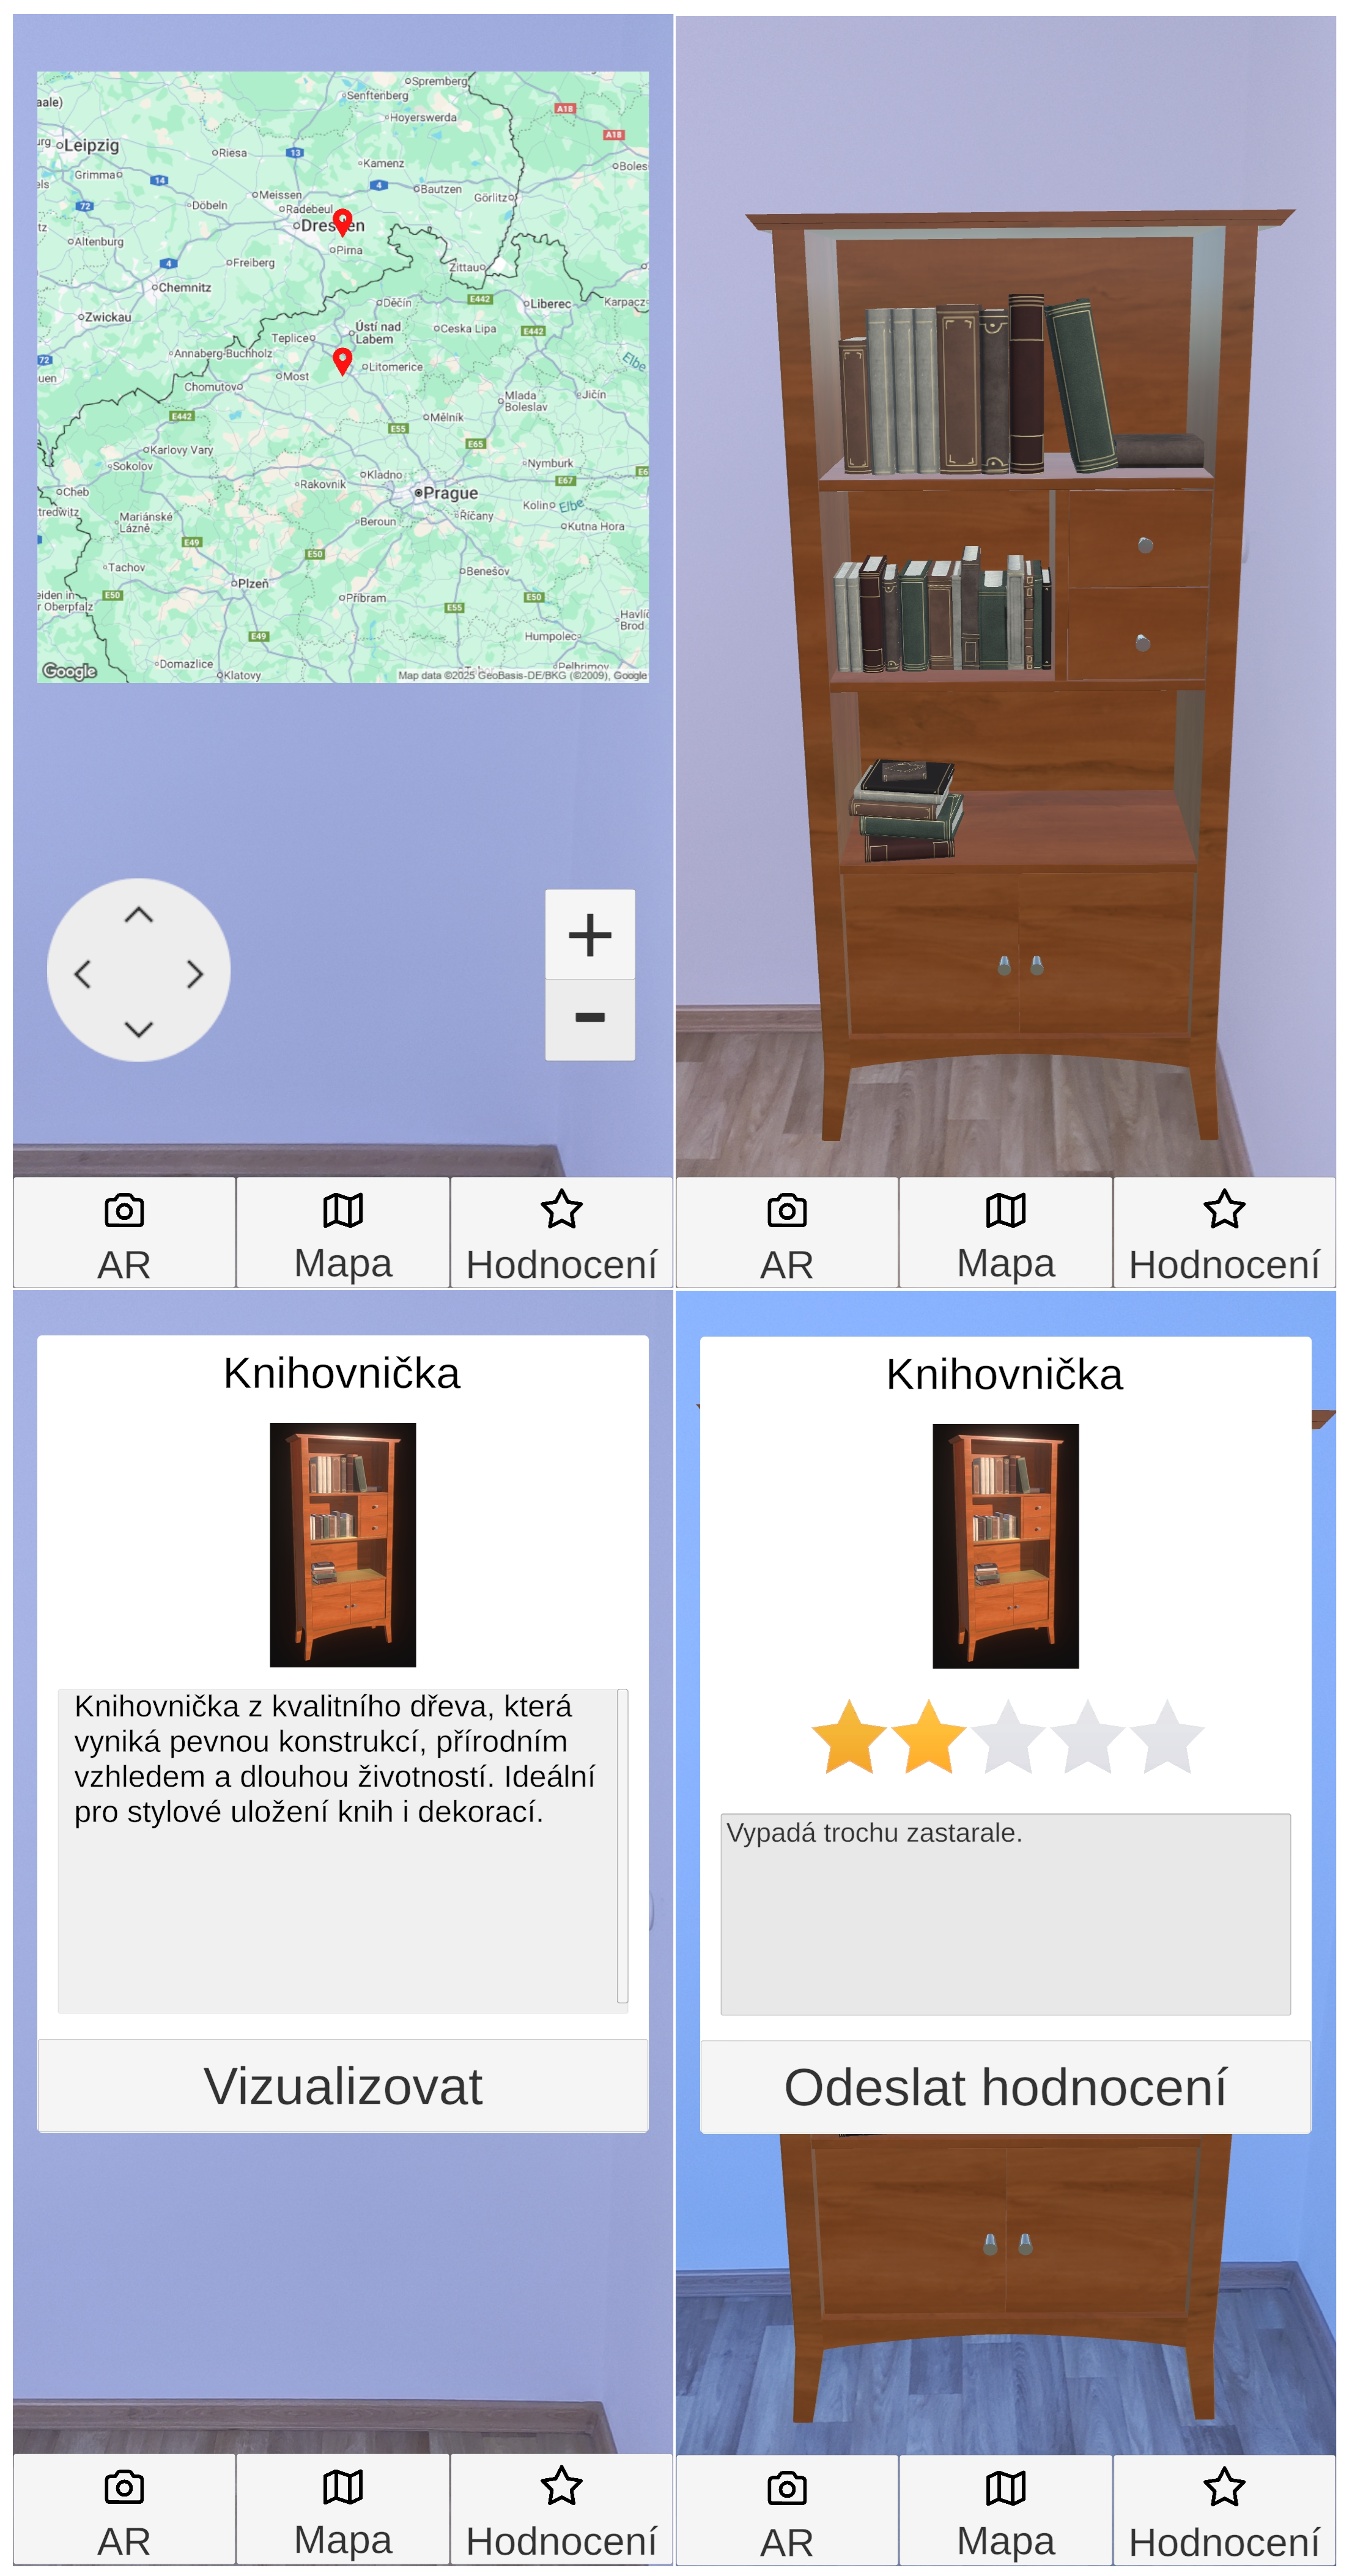
\includegraphics[width=0.8\textwidth]{images/mobile-app-showcase.png}
    \caption{Ukázka jednotlivých obrazovek v mobilní aplikaci}
    \label{fig:map}
\end{figure}

\section{Hodnocení splnění cílů}

Hlavním cílem bylo vytvořit funkční prototyp pro zobrazení digitálních dvojčat v rozšířené realitě.

Mobilní aplikace umožňuje zobrazení 3D modelů v AR bez fyzických markerů, mapové rozhraní pro výběr projektů a zpětnou vazbu formou hodnocení a komentářů. Uživatelské rozhraní je intuitivní a aplikace je kompatibilní s Androidem.

Serverová část zajišťuje komunikaci přes REST API, správu digitálních dvojčat a implementuje cache mechanismus pro mapové dlaždice, což optimalizuje výkon a snižuje náklady na volání Google Maps API.

Webové rozhraní umožňuje správu projektů včetně nahrávání modelů, úprav a mazání. Webové rozhraní obsahuje také přehled všech projektů, který obsahuje všechny důležité údaje včetně zpětné vazby.

Během vývoje byly upraveny některé požadavky. Ukládání do osobního repozitáře bylo nahrazeno přímým načítáním ze serveru, což eliminuje zastaralá data a zjednodušuje architekturu. Skenování QR kódů nebylo implementováno, protože mapa opouští od nutnosti vylepovat QR kódy na reálná místa projektů. Detailní projektové informace (termíny, náklady, odpovědné firmy) nebyly zahrnuty, prototyp obsahuje obecný popis, který tyto informace může zahrnovat. V případě potřeby je datový model připraven na rozšíření. Otáčení modelu gestem nebylo implementováno, uživatel model prohlíží pohybem zařízení, což odpovídá přirozenému používání AR.
